\section{Introduction}
Ce projet de pilotage de projet DevOps a pour but de mettre en pratique les connaissances acquises lors du cours avec l'utilisation de Docker et la mise en place de plusieurs services. 2 exercices seront proposés dans ce rendu, à savoir les exercices VIII et IX.

\section{Architecture}
\subsection{Exercice VIII}
\subsubsection*{Architecture générale}
La figure \ref{fig:exo8} présente l'architecture générale de cet exercice. On y retrouve un fichier \verb|docker-compose.yml| qui permet de lancer les 2 services : \verb|app| et \verb|db|. Le service \verb|app| est le projet Spring Boot fourni. Le service \verb|db| est une base de données MySQL.

\subsubsection*{Types de réseaux}
Le réseau utilisé est le réseau \verb|bridge| de Docker. Il permet de créer un réseau privé pour les conteneurs. Les ports 3306 et 8080 sont exposés pour pouvoir accéder à la base de données et à l'application Spring Boot.
\subsubsection*{Types de stockages}
Le stockage utilisé est le stockage \verb|volume| de Docker, ici nommé \verb|db_data|. Il permet de créer un volume pour les conteneurs. Il est utilisé pour la base de données afin de pouvoir conserver les données même si le conteneur est supprimé.

\subsection{Exercice IX}
\subsubsection*{Architecture générale}
\subsubsection*{Types de réseaux}
\subsubsection*{Types de stockages}

\section{Conclusion}

\section{Annexes}

\begin{figure}[hbtp]
    \centering
    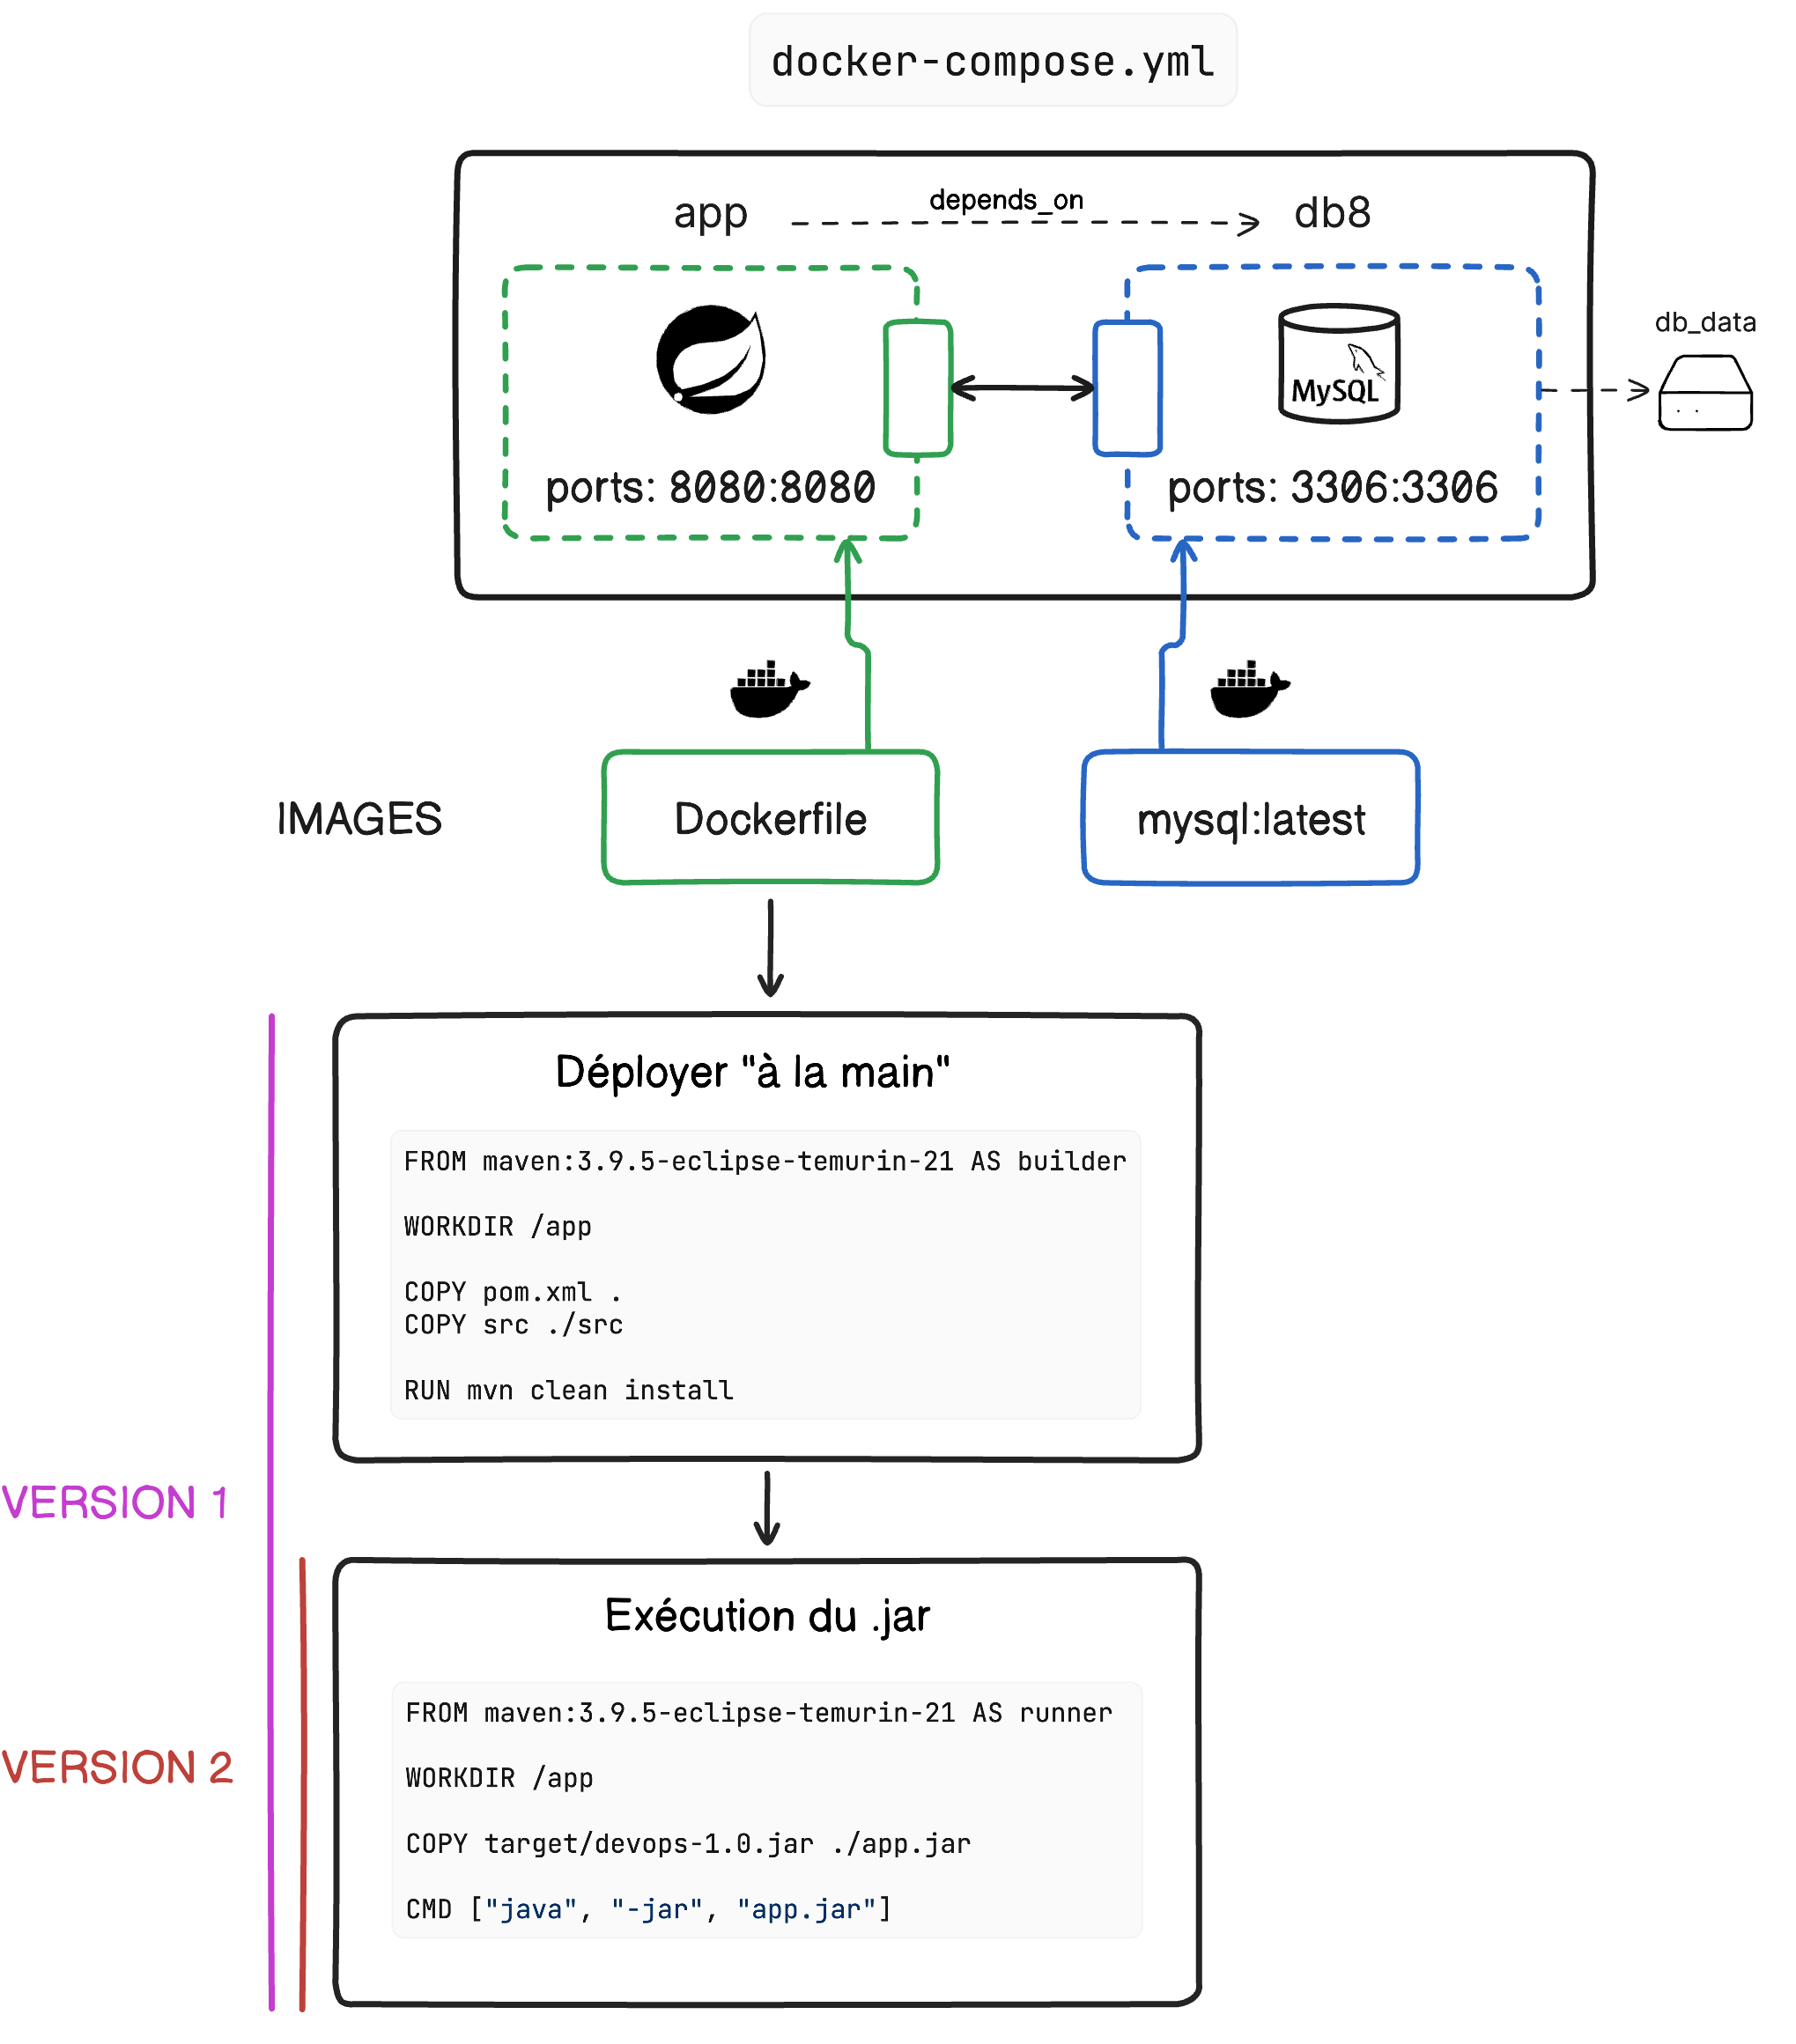
\includegraphics[width=\textwidth]{images/exo8.png}
    \caption{Architecture générale de l'exercice VIII}
    \label{fig:exo8}
\end{figure}